\section{Tangent lines}
Suppose we have two variables, $ y $ and $ x $, such that any change in $ x $ produces
a corresponding change in $ y $. In the language we learned last year, we say that $ y $
is a function of $ x $: that is, there is a function $ f $ such that $ y = f(x) $.

Let us look at a few different functions.

\begin{figure}\centering
  \begin{tikzpicture}
    \begin{axis}[
        axis lines = center,
        xlabel = $ x $,
        ylabel = {$ y = x^2 + x - 1 $}
      ]
        \addplot[domain = -5:5, color = red] {x^2 + x - 1};
    \end{axis}
  \end{tikzpicture}
  \caption{A parabola, $ y = x^2 + x - 1 $.\label{fig:func1}}
\end{figure}

Firstly, let's consider the function $ f $ defined by $ f(x) = x^2 + x - 1 $, graphed in figure \ref{fig:func1}. Let's
look at how $ f $ behaves at a point $ x_0 $ by adding a small number $ h $ to the input and seeing how it changes
the output.

\begin{displaymath}
  f(x_0 + h) = (x_0 + h)^2 + (x_0 + h) - 1 = x_0^2 + 2x_0 h + h^2 + x_0 + h - 1.
\end{displaymath}

We're actually interested in the difference between our new output and our old output, because this gives us
a measure of how quickly $ f $ changes when we move along the $ x$-axis by $ h $.

\begin{displaymath}
  f(x_0 + h) - f(x_0) = (x_0^2 + 2x_0 h + h^2 + x_0 + h - 1) - (x_0^2 + x_0 - 1) = 2x_0 h + h + h^2
\end{displaymath}

If $ h $ is small, then $ h^2 $ is miniscule and only makes up a very small part of $ f(x_0 + h) $. We can therefore
make the following approximation:
\begin{displaymath}
  f(x_0 + h) - f(x_0) \approx (2x_0 + 1)h.
\end{displaymath}
In other words, a small change in the input from $ x_0 $ to $ x_0 + h $ produces a change in the output of the form $ (2x_0 + 1)h $.

When we looked at straight lines in the past, they had a measure of \emph{slope}: the ratio of `rise' (change in output) to `run'
(change in input). For each $ x_0 $ that we feed into $ f $ here, we have a measure of the `rise' of $ f $ over a very small distance, $ h $.
It makes sense, then, to define the slope of $ y = f(x) $ at $ x_0 $ to be $\text{rise}/\text{run}$:
\begin{equation}
  \frac{f(x_0 + h) - f(x_0)}{h} \approx \frac{(2x_0 + 1)h}{h} = 2x_0 + 1
\end{equation}
So when $ h $ is very small, the graph of $ f $ between $ x_0 $ and $ x_0 + h $ looks like a straight line with slope $ 2x_0 + 1 $.

Since the slope of our function defined in this way depends on the value of $ x_0 $, we have a new function which assigns to each point $ x_0 $
the slope of $ f $ around $ x_0 $. We denote this function by $ f' $, and call it the \emph{derivative} of $ f $. The slope of $ f $ at $ x_0 $
will be written $ f'(x_0) $.

Another notation for the derivative is also common; because we are looking at changes in $ y $ divided by changes in $ x $ it sometimes
makes sense to write the derivative as $ \od{y}{x} $ (where $ \dif{x} $ denotes, in some sense, a small change in $ x $). The value of the
derivative at $ x_0 $ is written as $ \eval{\dod{y}{x}}_{x = x_0} $. This notation is known as Leibniz notation, as it was first introduced
in the 1600s by Gottfried Leibiz (a German mathematician and philosopher who, it can be argued, was one of the first modern mathematicians
to develop calculus in a sophisticated manner).

The derivative of the derivative of $ f $ is called the second derivative of $ f $, and we write $ f'' $ for this new function. In general,
the $ n$th derivative of $ f $ is denoted by $ f^{(n)} $ (it is the function produced by repeatedly differentiating $ f $). In Leibniz
notation, the $ n$th derivative of $ y = f(x) $ is $ \od[n]{y}{x} $.

\begin{defn}
  \begin{enumerate}
    \item If we can approximate the change in a function $ f $ around a point $ x_0 $ by writing $ f(x_0 + h) - f(x_0) \approx m h $
          for some constant $ m $ that depends on $ x_0 $ but not $ h $, then $ f $ is said to be differentiable at $ x_0 $
          with derivative $ m = f'(x_0) $.
    \item If $ y = f(x) $, then $ \od{y}{x} = f'(x) $.
    \item The line passing through $ (x_0,f(x_0)) $ with slope $ f'(x_0) $ is called the \emph{tangent line} to $ f $ at $ x_0 $.
  \end{enumerate}
\end{defn}

We will look at a more complicated function now. Consider $ y = \sin(x) $; we want to find its derivative, so we look at our
output difference:
\begin{displaymath}
  \sin (x + h) - \sin x = 2\cos \frac{(x + h) + x}{2} \sin \frac{(x + h) - x}{2} = 2\cos \left(x + \frac{h}{2} \right) \sin \left( \frac{h}{2} \right).
\end{displaymath}
For very small values of $ \alpha $, we have that $ \sin \alpha \approx \alpha $ (as long as we measure $ \alpha $ in radians).\footnote{See 2.13
in the trigonometry notes.} In particular, $ \sin(h/2) \approx h/2 $. Further, if $ h $ is very small then $ x + h/2 \approx x $. Making these
two approximations, we find that
\begin{displaymath}
  \sin (x + h) - \sin x \approx 2\cos(x) \cdot (h/2) = \cos(x) h.
\end{displaymath}
Thus, for each $ x $, we have
\begin{equation}
  \frac{\sin (x + h) - \sin x}{h} \approx \cos x;
\end{equation}
and as this approximation becomes arbitrarily precise as $ h $ gets closer to zero (because the closer $ h $ is to zero our
approximations $ h/2 \approx 0 $ and $ \sin(h/2) \approx h/2 $ become better and better) we feel justified in saying that $ \sin' = \cos $.

Finally, we will look at the absolute value function $ x \mapsto \abs{x} $ defined by
\begin{displaymath}
  \abs{x} = \begin{cases*} x & when $ x \geq 0 $; \\ -x & when $ x < 0 $ \end{cases*}.
\end{displaymath}
This function is graphed in figure \ref{fig:func3}.

\begin{figure}\centering
  \begin{tikzpicture}
    \begin{axis}[
        axis lines = center,
        xlabel = $ x $,
        ylabel = {$ y = \abs{x} $}
      ]
        \addplot[domain = -5:0, color = red] {-x};
        \addplot[domain = 0:5, color = red] {x};
    \end{axis}
  \end{tikzpicture}
  \caption{The absolute value function.\label{fig:func3}}
\end{figure}

Let's try to calculate the slope of $ y = \abs{x} $.

\begin{itemize}
  \item When we look around any positive $ x $, the definition tells us that $ \abs{x + h} = x + h $.
        Thus $ \abs{x + h} - \abs{x} = x + h - x = h $; hence $ \frac{\abs{x + h} - \abs{x}}{h} = 1 $,
        and so the derivative for any positive $ x $ is $ 1 $.
  \item When we look around any negative $ x $, the definition tells us that $ \abs{x + h} = - x - h $.
        Thus $ \abs{x + h} - \abs{x} = -x - h - (-x) = -h $; hence $ \frac{\abs{x + h} - \abs{x}}{h} = -1 $,
        and so the derivative for any negative $ x $ is $ -1 $.
\end{itemize}

But now we have a problem: at zero, if we take $ h $ to be a small positive number we find that $ \frac{\abs{x + h} - \abs{x}}{h} = 1 $;
but if $ h $ is a small negative number, then $ \frac{\abs{x + h} - \abs{x}}{h} = -1 $. Since looking in different directions from the same point
gives us different slopes, there is no good linear approximation to the curve $ y = \abs{x} $ at the point $ (0,0) $. We will
say that the curve is \emph{non-differentiable} there.

\subsection{Exercises and Problems}
\begin{enumerate}
  \item Let $ f $ be a function. Describe the difference between $ f $, $ f' $, $ f(57) $, and $ f'(57) $.
  \item The following data are temperatures $ T $ in a place measured hourly ($ t $ is the number of hours since noon, and $ T $ is measured
        in degrees celsius).

        \begin{tabular}{r|ccccccc}
          $ t $ & 0 & 2 & 4 & 6 & 8 & 10 & 12\\
          $ T $ & 15 & 16 & 16 & 15 & 14 & 13 & 13.
        \end{tabular}

        Since $ T $ is a function of $ t $, we can consider the derivative $ T' $. What does this derivative represent?
        What are the units of $ T'(t) $? Give an approximate value for $ T'(8) $.

  \item A particle is moving along a straight line, such that its displacement at time $ t $ is $ s(t) $ (in metres, measured from some starting point).
    \begin{enumerate}
      \item If $ t $ is measured in seconds, what are the units of $ s'(t) $? What is the meaning of this quantity?
      \item The derivative of $ s' $ is denoted by $ s'' $. What are the units of $ s''(t) $, and what is the meaning of this derivative?
    \end{enumerate}
  \item Consider the curve $ y = f(x) $ for some function $ x $. What is the equation of the line
        joining the points $ (x, f(x)) $ and $ (x + h, f(x + h)) $? By letting $ h $ approach zero,
        give a justification for the definition of the tangent line to $ f $ at $ (x,f(x)) $. (Include a picture!)
  \item The slope of a curve at a point tells us two things: whether it is sloping up or down, and the speed at which it is changing. Here
        are a few graphs of functions; sketch the graphs of their derivatives.
    \begin{multicols}{2}
    \begin{enumerate}
      \item
        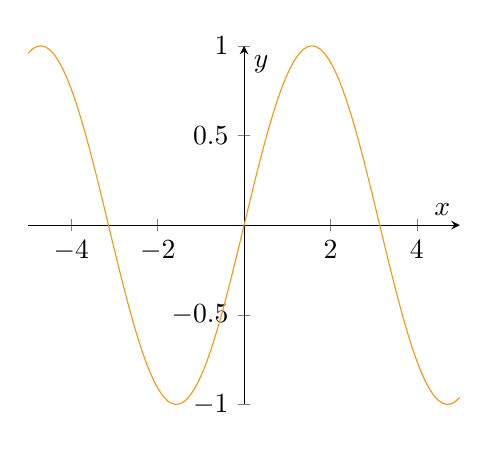
\begin{tikzpicture}
          \begin{axis}[
            axis lines = center,
            xlabel = $ x $,
            ylabel = $ y $,
            scale = .8
          ]
            \addplot[domain = -5:5, color = YellowOrange, samples=100] {sin(deg(x))};
          \end{axis}
        \end{tikzpicture}
      \item
        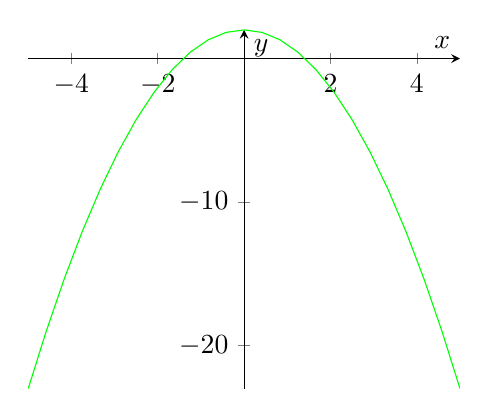
\begin{tikzpicture}
          \begin{axis}[
            axis lines = center,
            xlabel = $ x $,
            ylabel = $ y $,
            scale = .8
          ]
            \addplot[domain = -5:5, color = green] {-x^2 + 2};
          \end{axis}
        \end{tikzpicture}
      \item
        \begin{tikzpicture}
          \begin{axis}[
            axis lines = center,
            xlabel = $ x $,
            ylabel = $ y $,
            scale = .8
          ]
            \addplot[domain = -5:5, color = red, samples=100] {0.02*x^5 - 0.5*x^3 + x^2 - sin(x)};
          \end{axis}
        \end{tikzpicture}
      \item
        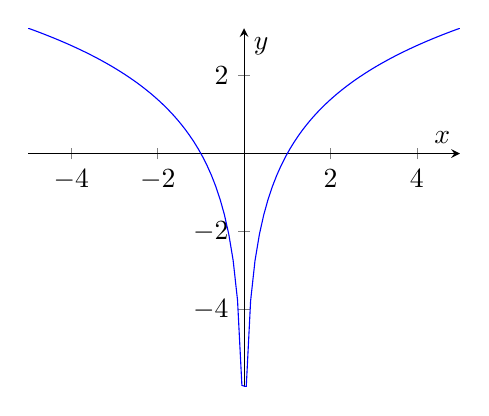
\begin{tikzpicture}
          \begin{axis}[
            axis lines = center,
            xlabel = $ x $,
            ylabel = $ y $,
            scale = .8
          ]
            \addplot[domain = -5:5, color = blue, samples=100] {ln(x^2)};
          \end{axis}
        \end{tikzpicture}
    \end{enumerate}
    \end{multicols}
  \item Describe several ways in which a function $ f $ can fail to be differentiable at a point $ x $, illustrating your examples with sketches.
  \item Consider each of these functions in turn. Where is the derivative of each (i) negative, (ii) positive, (iii) zero, and (iv) undefined?
    \begin{enumerate}
      \item $ x \mapsto x^2 $
      \item $ x \mapsto \sin x $
      \item $ x \mapsto \tan x $
    \end{enumerate}
  \item Justify: `The derivative of $ f $ is the same as the derivative of $ f + K $ for every constant $ K $.'\footnote{Here, $ f + K $ denotes
        the function defined by $ (f + K)(x) = f(x) + K $ for all $ x $. Likewise, if $ f $ and $ g $ are functions we define $ f + g $ to
        be the function satisfying $ (f + g)(x) = f(x) + g(x) $ for all $ x $.}
  \item Above, we proved that if $ y = x^2 + x - 1 $ then $ \od{y}{x} = 2x + 1 $. Write the equation of the
        tangent line to this curve at the point $ (3, 11) $.
  \item Let $ f $ be a function. Suppose that it is known that $ f'(3) = 9 $, and $ f(3) = 6 $.
    \begin{enumerate}
      \item What does the graph of $ y = f(x) $ look like around $ x = 3 $?
      \item Give the equation of the tangent line to $ f(x) $ at $ x = 3 $.
    \end{enumerate}
  \item The number of bacteria after $ t $ hours in a controlled laboratory experiment is $ n = f(t) $.
    \begin{enumerate}
      \item What is the meaning of the derivative $ f'(5) $?
      \item Suppose that there is an unlimited amount of space and nutrients. Which would you
            expect to be larger, $ f'(5) $ or $ f'(10) $? If the supply of nutrients is limited
            does your answer change?
    \end{enumerate}
  \item Prove that the only curves with constant slope are straight lines.
  \item A ball dropped from a tower accelerates from rest at a constant rate, $ -g $. If $ h(t) $ is the height of the ball $ t $ seconds
        after it is dropped, what is its velocity $ t $ seconds after being dropped?
  \item One model of population claims that the rate of change of a population $ P $ at a time is directly proportional to the size of
        the population at that time. In other words, $ \od{P}{t} = kP(t) $ for some constant $ P $. If $ P(0) = 100 $, sketch
        the population over time.
  \item Consider an ellipse, $ \frac{x^2}{a^2} + \frac{y^2}{b^2} = 1 $. This is not a function: since both $ (0, b) $ and $ (0, -b) $ are
            members of the function, it fails the vertical line test. However, it would be nice to reason about its
            rate of change \textit{as if it were} a function. Describe the slope of the ellipse as a particle traces the curve in
            an anticlockwise direction at a constant rate.
  \item If $ f(x) = x^3 + x $, calculate the derivative $ f' $ by writing $ f(x + h) - f(x) \approx kh $ for some $ k $.
  \item We will calculate the derivative of $ f(x) = \sqrt{x} $ at the point $ (1,1) $. To do this,
        consider the point $ P = (1,1) $ and the sequence of points $ P_h = (1 + 1/h, \sqrt{1 + 1/h}) $.
    \begin{enumerate}
      \item Justify: we will obtain the tangent line to $ f $ at $ P $ by taking $ h $ larger and larger, so $ P_h $
            gets closer and closer to $ P $.
      \item Show that the slope of the line joining $ P $ and $ P_h $ is $ \sqrt{h(h + 1)} - h $.
      \item Unfortunately, it is hard to see how this quantity behaves as $ h $ grows. Use the identity
            $ a^2 - b^2 = (a + b)(a - b) $ to rewrite $ \sqrt{h(h + 1)} - h $ as $ \frac{h(h + 1) - h^2}{\sqrt{h(h + 1)} + h} $.
      \item Rewrite this fraction as $ \frac{1}{\sqrt{1 + 1/h^2} + 1} $ (so $ \frac{f(1 + 1/h) - f(x)}{1/h} = \frac{1}{\sqrt{1 + 1/h^2} + 1} $),
            and hence show that $ f'(1) = 1/2 $.
    \end{enumerate}
\end{enumerate}

\subsection{References}
For a readable introduction to differentiation as the study of linear approximations analagous
to what we see above, see the first few chapters of Thompson's \emph{Calculus made easy}.

For many exercises on the behaviour of derivatives (as rates of change, and as slopes of tangent
lines) see sections 2.1 and 2.2 of Stewart.

See also the section on calculus from my L2 notes.

\subsection{Homework}
\paragraph{Reading}
Considering how many fools can calculate, it is surprising that it should be thought a difficult or
a tedious task for any other fool to learn how to master the same tricks.

Some calculus-tricks are quite easy. Some are enormously difficult. The fools who write the text-books
of advanced mathematics --- and they are mostly clever fools --- seldom take the time to show you how
easy the easy calculations are. On the contrary, they seem to desire to impress you with their tremendous
cleverness by going about it in the most difficult way.

Being myself a remarkably stupid fellow, I have had to unteach myself the difficulties, and now beg
to present to my fellow fool the parts that are not hard. Master these thoroughly, and the rest will
follow. What one fool can do, another can.

The preliminary terror, which chokes off most high school students from even attempting to learn
how to calculate, can be abolished once and for all by simply stating what is the meaning --- in
common-sense terms --- of the two principal symbols that are used in calculating.

These dreadful symbols are:

(1) $ \dif{} $, which merely means ``a little bit of''.

Thus $ \dif{x} $ meas a little bit of $ x $;
or $ \dif{u} $ means a little bit of $ u $. Ordinary mathematicians think it more polite to say
``an element of'', instead of ``a little bit of''. Just as you please. But you will find that these
little bits (or elements) may be considered to be infinitesimally small.

(2) $ \rint $, which is merely a long $ S $, and may be called (if you like) ``the sum of''.

Thus $ \rint \dif{x} $ means the sum of all the little bits of $ x $; or $ \rint \dif{t} $ means
the sum of all the little bits of $ t $. Ordinary mathematicians call this symbol ``the integral of''.
Now any fool can see that if $ x $ is considered to be made up of a lot of little bits, each of
which is called $ \dif{x} $, if you add them all up together you get the sum of all the $ \dif{x}$'s (which
is simply the same thing as the whole of $ x $). The word ``integral'' simply means ``the whole''. If you think
of the duration of time for one hour, you may  (if you like) think of it cut up into 3600 little bits
called seconds. The whole of the 3600 little bits added up together make one hour.

When you see an expression that begins with this terrifying symbol, you will henceforth know that it is put
there merely to give you instructions that you are now to perform the operation (if you can) of totalling up
all the little bits that are indicated by the symbols that follow.

That's all.

\begin{flushright}
  From \textit{Calculus made easy}, by Silvanus P. Thompson and revised by Martin Gardner.
\end{flushright}

\paragraph{Problems}
\begin{enumerate}
  \item Draw the derivative of the following graphed function:
        \begin{center}
        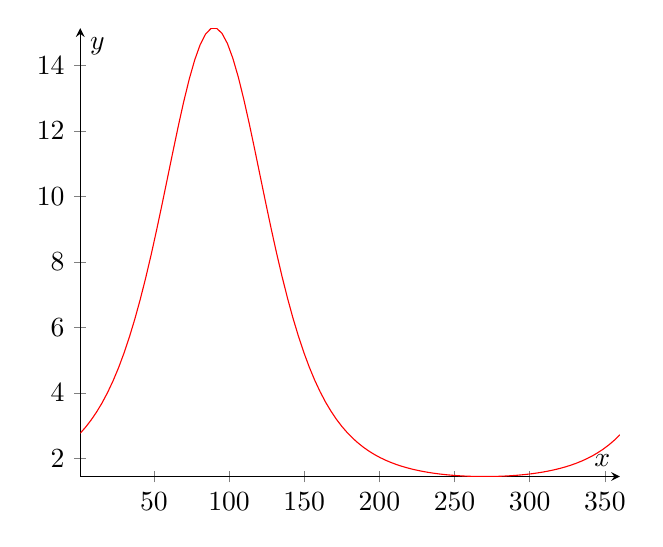
\begin{tikzpicture}
          \begin{axis}[
            axis lines = center,
            xlabel = $ x $,
            ylabel = $ y $
          ]
            \addplot[domain = 1:360, color = red, samples=100] {exp(exp(sin(x)))};
          \end{axis}
        \end{tikzpicture}
        \end{center}
  \item The following is the graph of the derivative of some function $ f $. Sketch the graph of $ f $, if $ f(0) = 0 $.
        \begin{center}
        \begin{tikzpicture}
          \begin{axis}[
            axis lines = center,
            xlabel = $ x $,
            ylabel = $ y $
          ]
            \addplot[domain = 0:10, color = red, samples=100] {1/(x + 1) - 0.5};
          \end{axis}
        \end{tikzpicture}
        \end{center}
  \item Show that if $ f $ and $ g $ are two functions, then $ (f + g)' = f' + g' $.
\end{enumerate}
